\documentclass[a4paper,12pt]{article}

\usepackage{a4wide}
\usepackage{amsfonts}
\usepackage{amsmath}
\usepackage{amssymb}
\usepackage{lipsum}

\usepackage{graphicx}  % For including images

\usepackage{xcolor}  % For a colorfull presentation
\usepackage{listings}  % For presenting code 

\usepackage{hyperref}

% Definition of a style for code, matter of taste
\lstdefinestyle{mystyle}{
  language=Python,
  basicstyle=\ttfamily\footnotesize,
  backgroundcolor=\color[HTML]{F7F7F7},
  rulecolor=\color[HTML]{EEEEEE},
  identifierstyle=\color[HTML]{24292E},
  emphstyle=\color[HTML]{005CC5},
  keywordstyle=\color[HTML]{D73A49},
  commentstyle=\color[HTML]{6A737D},
  stringstyle=\color[HTML]{032F62},
  emph={@property,self,range,True,False},
  morekeywords={super,with,as,lambda},
  literate=%
    {+}{{{\color[HTML]{D73A49}+}}}1
    {-}{{{\color[HTML]{D73A49}-}}}1
    {*}{{{\color[HTML]{D73A49}*}}}1
    {/}{{{\color[HTML]{D73A49}/}}}1
    {=}{{{\color[HTML]{D73A49}=}}}1
    {/=}{{{\color[HTML]{D73A49}=}}}1,
  breakatwhitespace=false,
  breaklines=true,
  captionpos=b,
  keepspaces=true,
  numbers=none,
  showspaces=false,
  showstringspaces=false,
  showtabs=false,
  tabsize=4,
  frame=single,
}
\lstset{style=mystyle}

\begin{document}
\title{Machine Learning A (2023)\\Home Assignment 2}
\author{\color{red}Niels Moctezuma Krarup. Student ID: WTG176}
\date{}
\maketitle

% Please leave the table of contents as is, for the ease of navigation for TAs
\tableofcontents % Generates the table of contents
\newpage % Start a new page after the table of contents

\section{Illustration of Markov's, Chebyshev's, and Hoeffding's Inequalities (24 points)}

\subsection*{2a}
\subsubsection*{1}
We start by plotting the empirical distribution based on 1e6 replications of observing the mean being above $\alpha \in \{0.5, 0.55,\dots , 0.95, 1\}$.

% Placeholder figure
\begin{figure}[htbp]
    \centering
    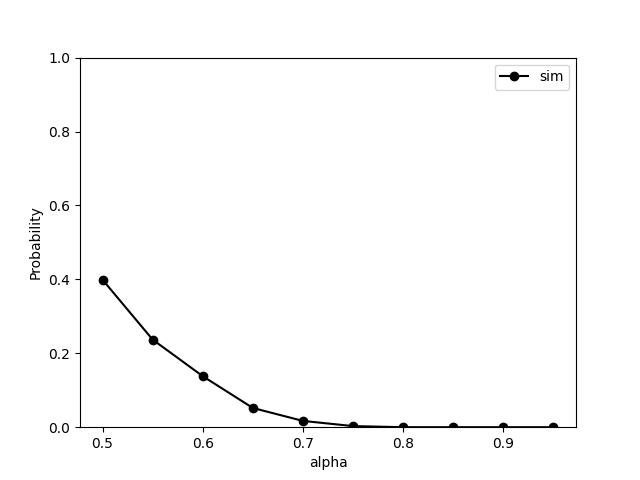
\includegraphics[width=0.5\linewidth]{HA2_2a_1.png}
    \caption{simulated frequencies of surpassing alpha} % Dummy caption generated using lipsum
    \label{fig:1}
\end{figure}



\subsubsection*{2}
Since we take the mean of 20 Bernoulli random variables, the mean will only take on 21 different values, i.e. it will live on the space $\{0, \frac{1}{20},\dots , 1\}$. Due to having increments of size $\frac{1}{20}$ from adding another 'success' from one of the 20 realisations. Hence nothing new will be happening between the steps defined in the $\alpha$ vector. Of course if we were to increase $n$ this would change, as the mean would be more fine-grained.

\subsubsection*{3}
From the theorem on Markov Bound we get, since the mean is non-negative and has 1st moment that
$$
\mathbb{P}\left( \frac{1}{n}\sum_{i = 1}^nX_i \geq \alpha \right) \leq \frac{\mathbb{E}\left[ \frac{1}{n}\sum_{i = 1}^nX_i \right]}{\alpha} = \frac{0.5}{\alpha}
$$

Where we have used linearity of the expected value (it is an intergral) and that the expected value of a bernouli random variable is $\mu = 0.5$.

Let's draw in these bounds. 
% Placeholder figure
\begin{figure}[htbp]
    \centering
    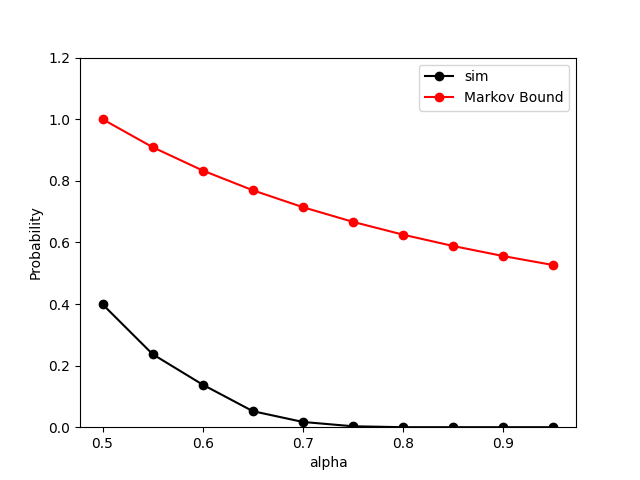
\includegraphics[width=0.5\linewidth]{HA2_2a_2.png}
    \caption{markov bounds with simulated frequencies of surpassing alpha} % Dummy caption generated using lipsum
    \label{fig:2}
\end{figure}

\subsubsection*{4}
From the theorem on Chebyshev’s Inequality we get, since the mean is symetric around its mean = 0.5 we get:

\begin{align}
&\mathbb{P}\left( \left| \frac{1}{n}\sum_{i = 1}^nX_i - 0.5 \right| \geq \epsilon  \right) \leq \frac{Var\left[ \frac{1}{n}\sum_{i = 1}^nX_i \right]}{\epsilon^2} \Leftrightarrow
\\
&2\mathbb{P}\left(  \frac{1}{n}\sum_{i = 1}^nX_i \geq \epsilon + 0.5 \right) \leq \frac{Var\left[ \frac{1}{n}\sum_{i = 1}^nX_i \right]}{\epsilon^2} \Leftrightarrow
\\
&\mathbb{P}\left(  \frac{1}{n}\sum_{i = 1}^nX_i \geq \epsilon + 0.5 \right) \leq \frac{p(1-p)}{2n\epsilon^2} \Leftrightarrow
\\
&\mathbb{P}\left(  \frac{1}{n}\sum_{i = 1}^nX_i \geq \epsilon + 0.5 \right) \leq \frac{0.25}{2n\epsilon^2}
\end{align}

Where we use that the variance of a bernouli random variable is $p(1-p1)$.\
Since we are asked to evaluate along the threshold of $\alpha = \{0.5, 0.55, \dots, 1\}$ we see that in the above we should let $\epsilon$ above range from $\{0, 0.05, \dots, 0.5 \}$. The bound is above 1 for some values, hence we take the trivial minimim of $1$ and the bound. That is, we plot
$$
\min\left( 1, \frac{0.25}{2n\epsilon^2} \right), \epsilon = 0, 0.05, \dots, 0.5.
$$

From which we get the below 
\begin{figure}[htbp]
    \centering
    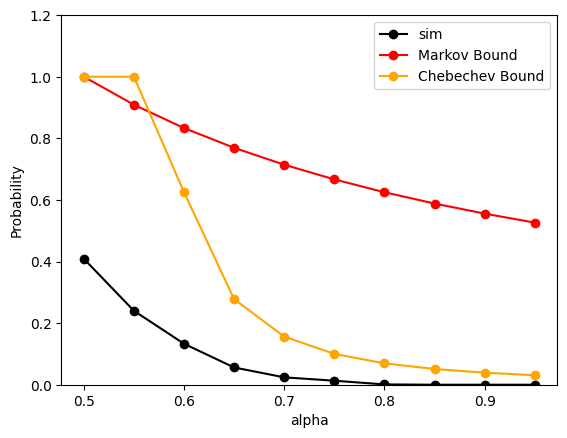
\includegraphics[width=0.5\linewidth]{HA2_2a_3.png}
    \caption{Markov- and Chebyshev’s bounds with simulated frequencies of surpassing alpha} % Dummy caption generated using lipsum
    \label{fig:2}
\end{figure}

\subsubsection*{5}
We use the one-sided  Hoeffding’s inequality, and get:
\begin{align}
\mathbb{P}\left(  \frac{1}{n}\sum_{i = 1}^nX_i \geq \alpha \right) =  
&\mathbb{P}\left(  \frac{1}{n}\sum_{i = 1}^nX_i - 0.5 \geq \underbrace{\alpha - 0.5}_{\epsilon} \right) \leq e^{-2n\epsilon^2}
\end{align}

From which we get the below 
\begin{figure}[htbp]
    \centering
    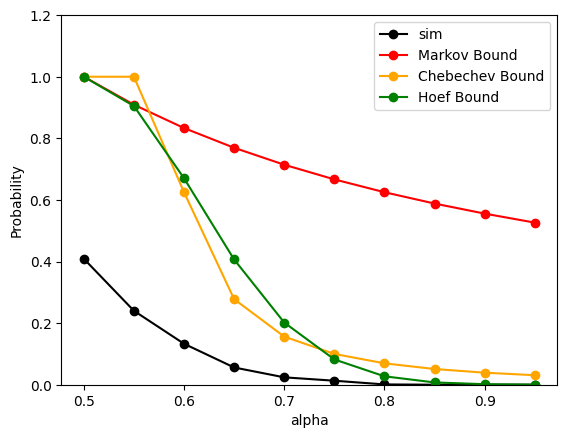
\includegraphics[width=0.5\linewidth]{HA2_2a_4.png}
    \caption{Markov, Chebyshev’s- and  Hoeffding’s bounds with simulated frequencies of surpassing alpha} % Dummy caption generated using lipsum
    \label{fig:3}
\end{figure}

\subsubsection*{6}
In the following we consider $n$ fixed and instead focus on the threshold, $\alpha$, ie how far from the theoretical true $\mu$, which in this ML case is then the error rate of our classifier that is the mean loss.
Comparing the plots and the shape of the 3 bounds and how they relate to the simulated probabilities we clearly see the that the markov bound is decreasing slowly by the rate $\frac{1}{\alpha}$ whereas the Chebechev bound decreases by $\frac{1}{\alpha^2}$, and lastly the Hoeffdinger bound decreases exponentially fast $e^{-\alpha^2}$.

Of course exponential decay is always faster than linear, but only in the limit, hence, as we see in the plot, one can not say that one is better than the other but in the limit is seems that the Hoeffdings bound is the strongest bound.

In any case one can calculate all three bounds and use the lower

\subsubsection*{7}
For the mean to be greater than or equal to $\alpha = 1$ we would need all the bernouli rvs to be $1$. Since each has probability $p = 0.5$ of doing this, the probability is simply
$$
\mathbb{P}\left(  \frac{1}{n}\sum_{i = 1}^nX_i \geq 1 \right) = 0.5^{20} = 9.5367431640625e-07
$$
so something like 20 in a million chance.


similairly for $\alpha = 0.95$ all but one would need to be loss, i.e 19 $X_i = 1$ and one $X_j = 0$
this happens with probability given below, plus the case from  above.
$$
\mathbb{P}\left(  \frac{1}{n}\sum_{i = 1}^nX_i \geq 1 \right) = p^{19}*(1-p)*20 + 0.5^20 = 2.002716064453125e-05
$$
so something like 1 in a million chance.

Python code to do the calculations:
% Placeholder code
\begin{lstlisting}
import scipy.stats as stats

#using cdf for bionomial dist.
tail_probability_1   = 1 - stats.binom.cdf(19, n, 0.5)
tail_probability_095 = 1 - stats.binom.cdf(18, n, 0.5)

print(tail_probability_1, tail_probability_095)

#by hand
res1 = p**20
res2 = p**19*p*20 + res1

print(res1, res2)
\end{lstlisting}

\subsubsection*{8}


\subsection*{2b}
%rep 1-7 above
\subsubsection*{1}
We start by plotting the empirical distribution based on 1e6 replications of observing the mean being above $\alpha \in \{0.5, 0.55,\dots , 0.95, 1\}$.

% Placeholder figure
\begin{figure}[htbp]
    \centering
    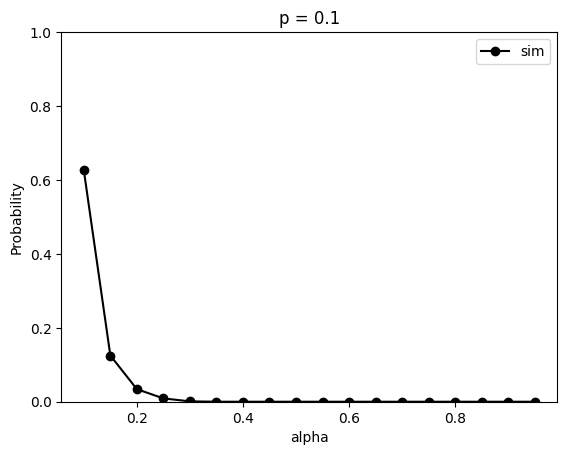
\includegraphics[width=0.5\linewidth]{HA2_2a_21.png}
    \caption{simulated frequencies of surpassing alpha (p = 0.1)} % Dummy caption generated using lipsum
    \label{fig:p01}
\end{figure}


\subsubsection*{3}
Markov bound
% Placeholder figure
\begin{figure}[htbp]
    \centering
    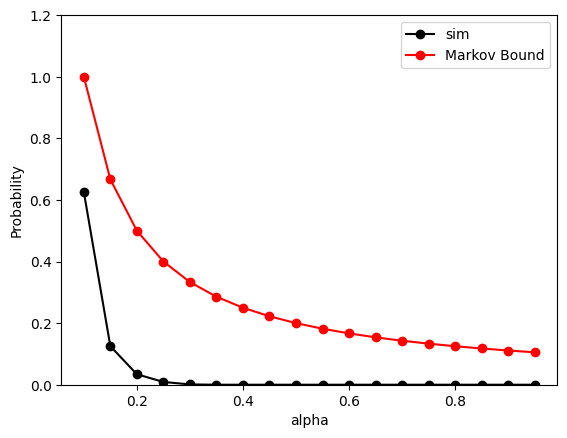
\includegraphics[width=0.5\linewidth]{HA2_2a_22.png}
    \caption{simulated frequencies of surpassing alpha (p = 0.1)} % Dummy caption generated using lipsum
    \label{fig:p01}
\end{figure}

\subsubsection*{4}
Chebechev bound
% Placeholder figure
\begin{figure}[htbp]
    \centering
    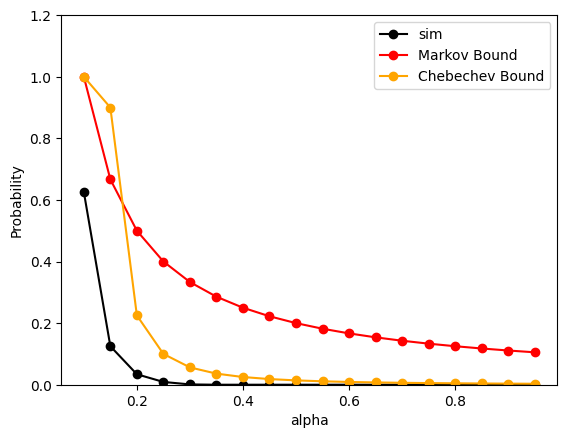
\includegraphics[width=0.5\linewidth]{HA2_2a_23.png}
    \caption{Markov- and Chebyshev’s bounds with simulated frequencies of surpassing alpha (p = 0.1)} % Dummy caption generated using lipsum
    \label{fig:p01}
\end{figure}

\subsubsection*{5}
Hoeffding bound
% Placeholder figure
\begin{figure}[htbp]
    \centering
    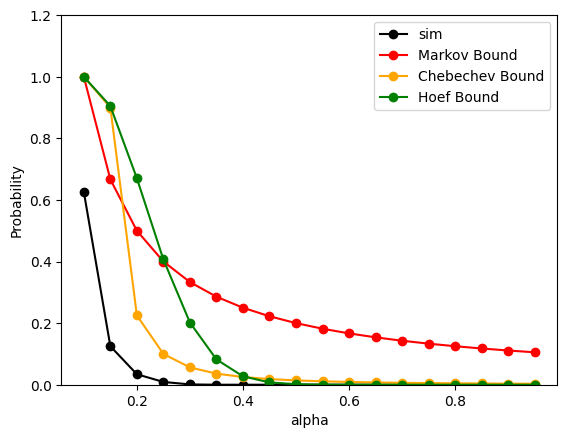
\includegraphics[width=0.5\linewidth]{HA2_2a_24.png}
    \caption{Markov, Chebyshev- and Hoeffding's bounds with simulated frequencies of surpassing alpha (p = 0.1)} % Dummy caption generated using lipsum
    \label{fig:p01}
\end{figure}


\subsubsection*{6}
The bounds are now much lower. This is because the mean (and the variance) is smaller.
intuitively it also makes sense now. Our algorithm only makes error with rate 0.1, hence we are much more confident in the loss being close to the expected.


\subsubsection*{7}
The probabilities from before are now practiaclly zero. I get:
\begin{lstlisting}

#by hand
res1 = p**20
res2 = p**19*p*20 + res1

print(res1, res2)

1.0000000000000011e-20 1.810000000000002e-18
\end{lstlisting}

So more or less zero. This makes sense as $p=0.1$ now.

\subsection*{2c}
%discussion
It should first be noted that in practise we do not have the values $\mu$ since this is unkown characteristic of the model.





\section{The Role of Independence (13 points)}
An easy but instrictive example is to make the $X_i$'s completely dependent of each other, that is $X_1 = X_n, n \geq 1$. \\
If we set $\mu = \mathbb{E} X_1 = 0.5$ then the mean will be either $0$ or $1$ for all $n \geq 1$ and the absolute difference to $\mu$ will hence be $\frac{1}{2}$ with probability $1$. 

Note that if we let $\mu \in (0,1)$ then the difference will only be greater than $\frac{1}{2}$ if the less likely outcome happens:
$$
\mathbb{P}\left( | \mu - \frac{1}{n}\sum_{i = 1}^n X_i  |   \geq \frac{1}{2} \right)  = \min(\mu, 1-\mu)
$$

\section{Tightness of Markov’s Inequality (Optional, question not for submission, 0 points)}

Take a random variable $X$ which has distribution such that the median and mean are not proportional of each other. Then one can scale the mean such that it is half as big as the median then by definition the probability of X being larger than its median is 0.5, and the markov bound will be 1/2.

One could e.g. choose the lognormal distribution which has mean $e^{\mu + \sigma^2/2}$ and median $e^\mu$
then pick $\sigma = \sqrt{2\log{1/2}}$ now the markov bound is tight when evaluated in the median.
i.e.
$$
\mathbb{P}\left( X  \geq  e^\mu \right) \leq \frac{e^{\mu + \sigma^2/2}}{e^\mu} = \frac{1}{2}
$$


\section{The effect of scale (range) and normalization of random variables in Hoeffding's inequality (13 points)}


This follows simply from THM 2.3, since if $X_i \in [0,1]$ then we can set $a_i = 0, b_i = 1,\, \forall i = 1,...,n$.
By evaluating THM 2.3 in the threshol $n\epsilon$ it then reads:
\begin{align}
&\mathbb{P}\left(  \sum_{i = 1}^nX_i - \mathbb{E}\left[ \sum_{i = 1}^nX_i \right] \geq n\epsilon \right) \leq e^{-2(n\epsilon)^2 / \sum (b_i - a_i)^2}  \Leftrightarrow \\
&\mathbb{P}\left(  \frac{1}{n}\sum_{i = 1}^nX_i - \mu \geq \epsilon \right) \leq e^{-2n^2\epsilon^2 / n}
\end{align}
where we have used that $\mathbb{E}X_i = \mu$ for all $i = 1,...,n$ and linearity of the mean. Multiplied by $1/n$ on both sides of the inequality in the event, and that the sum in the exponent is simply a sum of 1s $n$times, hence it yields $n$.
Cleaning up we end up with
$$
\mathbb{P}\left(  \frac{1}{n}\sum_{i = 1}^nX_i - \mu \geq \epsilon \right) \leq e^{-2n\epsilon^2}
$$






\section{Linear Regression (50 points)}

\subsubsection*{1}
% Placeholder code
\begin{lstlisting}
import numpy as np

def linear_reg(x,y):
  if len(x.shape) == 0: raise ValueError('Need covariates!!')
  elif len(x.shape) == 1:
    n = x.shape[0] #take nrow
    d = 1 #num covariates
    X = np.ones((n,2)) #fill out ones. for replacement later
    X[:,0] = x #first col 
  else:
    n, d = x.shape #d > 1
    X = np.ones((n, d+1))
    X[:, :d] = x
  pseudo_inv_X = np.matmul( np.linalg.inv( np.matmul(X.T, X)), X.T) #(XTX)^-1 XT
  print(pseudo_inv_X.shape)
  reg_fit = np.matmul(pseudo_inv_X, y)
  w = reg_fit[:d]
  b = reg_fit[d:]
  return w,b

print(linear_reg(x=data[:,0], y=data[:,1]))

(array([1.55777052]), array([-1.45194395]))
\end{lstlisting}

the function return the weight $w_1 = 1.55777052$ (there is only one weight as $d=1$), as well as the  
intercept $b = -1.45194395$.


\subsubsection*{2}
We log-transforming the $y$ we in effect fit the non-linear model. 
We include a calculation of the mean squared error. i.e. mean of $(y_i - exp(ax_i+b)^2$


\begin{lstlisting}
def nonlinear_reg(x,y):
  if len(x.shape) == 0: raise ValueError('Need covariates!!')
  elif len(x.shape) == 1:
    n = x.shape[0] #take nrow
    d = 1 #num covariates
    X = np.ones((n,2)) #fill out ones. for replacement later
    X[:,0] = x #first col 
  else:
    n, d = x.shape #d > 1
    X = np.ones((n, d+1))
    X[:, :d] = x
  y_trans = np.log(y)
  pseudo_inv_X = np.matmul( np.linalg.inv( np.matmul(X.T, X)), X.T) #(XTX)^-1 XT
  reg_fit = np.matmul(pseudo_inv_X, y_trans)
  a = reg_fit[:d]
  b = reg_fit[d:]
  mse = np.mean((y - np.exp(a*x + b))**2)
  return a,b, mse

print(nonlinear_reg(x=data[:,0], y=data[:,1]))

(array([0.25912824]), array([0.03147247]), 34.83556116722035)
\end{lstlisting}

we get $a = 0.25912824$ and $b = 0.03147247$, the mean squared error is 34.83556116722035.


\subsubsection*{4}
When we use the fitted values above we get:
% Placeholder figure
\begin{figure}[htbp]
    \centering
    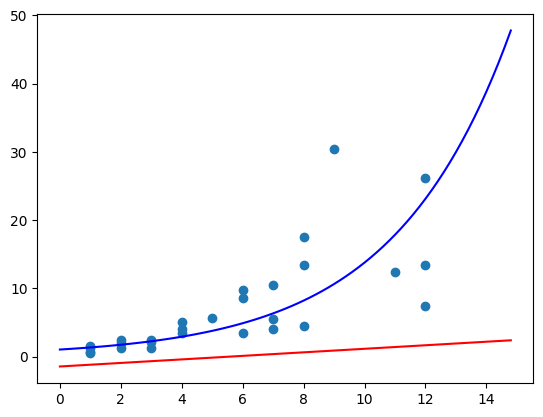
\includegraphics[width=0.5\linewidth]{reg_4.png}
    \caption{red:linear, dark blue: exp, blue: data} % Dummy caption generated using lipsum
    \label{fig:reg_1}
\end{figure}



\bibliography{bibliography}  % If you have some references, use BibTeX

\end{document}